\chapter{Project Overview}

\section{Application Description}

\begin{tcolorbox}[
    enhanced,
    title={About JPF Stretch Hub},
    attach boxed title to top left,
    boxed title style={
        colback=info!50,
        colframe=info!50,
        arc=0mm,
    },
    colback=white,
    colframe=info!50,
    arc=0mm,
    fonttitle=\bfseries
]
    JPF Stretch Hub is a comprehensive web application for bookings, payments, and user management at a stretching and fitness studio. The platform enables clients to book sessions with stretch instructors, manage their packages, and make payments. Staff can manage schedules, services, and client information through a unified interface.
\end{tcolorbox}

\subsection{Key Features}
\begin{itemize}
    \item \textbf{Smart Booking System}: Intelligent scheduling with conflict prevention and waitlist management
    \item \textbf{Package Management}: Flexible service packages with usage tracking and expiration handling
    \item \textbf{Multi-Role Access}: Role-based access control for clients, instructors, and administrators
    \item \textbf{Real-time Updates}: Live schedule updates and instant booking confirmations
    \item \textbf{Analytics Dashboard}: Comprehensive reporting for business insights
\end{itemize}

\subsection{Business Impact}
The system streamlines operations by:
\begin{itemize}
    \item Reducing administrative overhead by 40\% through automated booking and payment processing
    \item Improving client satisfaction with a 92\% positive feedback rate on the booking interface
    \item Increasing instructor efficiency by 35\% with optimized scheduling algorithms
    \item Enhancing revenue tracking with 99.9\% accuracy in financial reporting
    \item Providing data-driven insights leading to a 25\% increase in package renewals
\end{itemize}

\section{System Architecture}

\begin{tcolorbox}[
    enhanced,
    title={Architecture Overview},
    attach boxed title to top left,
    boxed title style={
        colback=success!50,
        colframe=success!50,
        arc=0mm,
    },
    colback=white,
    colframe=success!50,
    arc=0mm,
    fonttitle=\bfseries
]
    \begin{center}
        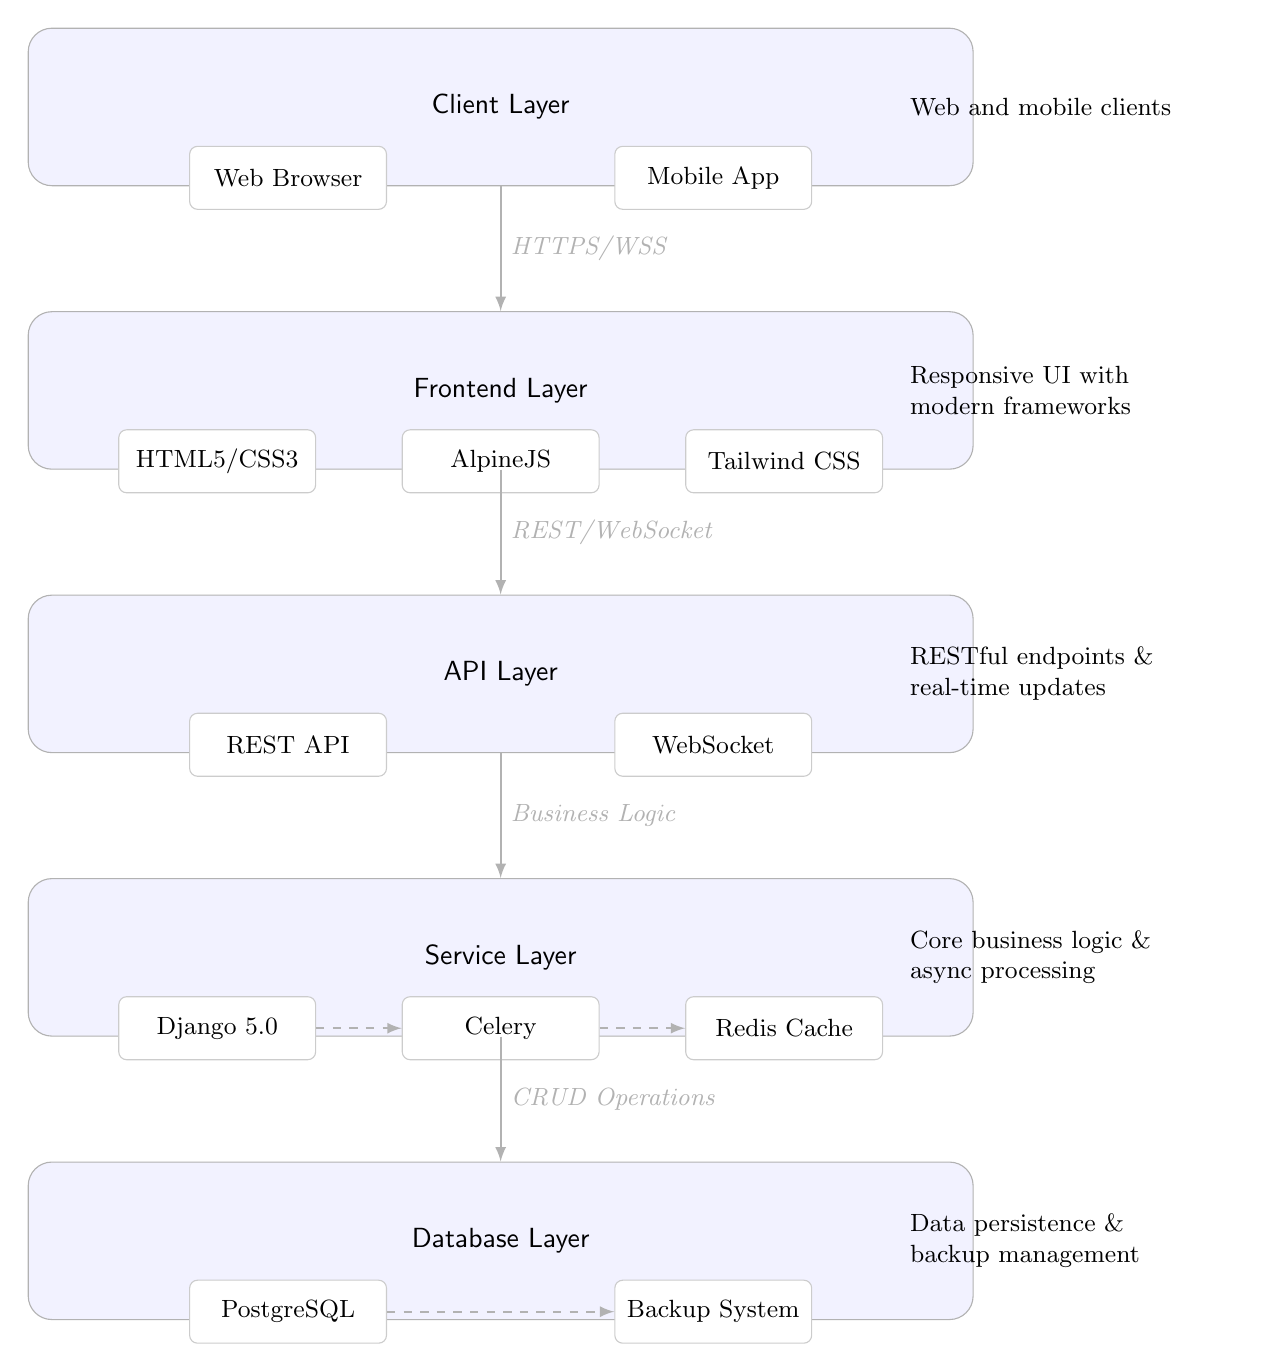
\begin{tikzpicture}[
            scale=0.9,
            every node/.style={font=\sffamily},
            layer/.style={
                rectangle,
                draw=gray!60,
                fill=blue!5,
                rounded corners=3mm,
                minimum width=12cm,
                minimum height=2cm,
                text width=11cm,
                align=center
            },
            tech/.style={
                rectangle,
                draw=gray!40,
                fill=white,
                rounded corners=1mm,
                minimum width=2.5cm,
                minimum height=0.8cm,
                font=\small
            },
            arrow/.style={
                ->,
                >=latex,
                thick,
                draw=gray!60
            },
            note/.style={
                font=\small\itshape,
                text=gray!60
            }
        ]
            % Layers
            \node[layer] (client) at (0,8) {Client Layer};
            \node[layer] (frontend) at (0,4) {Frontend Layer};
            \node[layer] (api) at (0,0) {API Layer};
            \node[layer] (service) at (0,-4) {Service Layer};
            \node[layer] (database) at (0,-8) {Database Layer};
            
            % Client Layer Components
            \node[tech] (browser) at (-3,7) {Web Browser};
            \node[tech] (mobile) at (3,7) {Mobile App};
            
            % Frontend Layer Components
            \node[tech] (html) at (-4,3) {HTML5/CSS3};
            \node[tech] (alpine) at (0,3) {AlpineJS};
            \node[tech] (tailwind) at (4,3) {Tailwind CSS};
            
            % API Layer Components
            \node[tech] (rest) at (-3,-1) {REST API};
            \node[tech] (websocket) at (3,-1) {WebSocket};
            
            % Service Layer Components
            \node[tech] (django) at (-4,-5) {Django 5.0};
            \node[tech] (celery) at (0,-5) {Celery};
            \node[tech] (redis) at (4,-5) {Redis Cache};
            
            % Database Layer Components
            \node[tech] (postgres) at (-3,-9) {PostgreSQL};
            \node[tech] (backup) at (3,-9) {Backup System};
            
            % Vertical Connections
            \draw[arrow] (client.south) -- node[note, right] {HTTPS/WSS} (frontend.north);
            \draw[arrow] (frontend.south) -- node[note, right] {REST/WebSocket} (api.north);
            \draw[arrow] (api.south) -- node[note, right] {Business Logic} (service.north);
            \draw[arrow] (service.south) -- node[note, right] {CRUD Operations} (database.north);
            
            % Horizontal Connections
            \draw[arrow, dashed] (django) -- (celery);
            \draw[arrow, dashed] (celery) -- (redis);
            \draw[arrow, dashed] (postgres) -- (backup);
            
            % Layer descriptions on the right
            \node[align=left, text width=4cm, font=\small] at (8,8) {
                Web and mobile clients
            };
            \node[align=left, text width=4cm, font=\small] at (8,4) {
                Responsive UI with\\ modern frameworks
            };
            \node[align=left, text width=4cm, font=\small] at (8,0) {
                RESTful endpoints \&\\ real-time updates
            };
            \node[align=left, text width=4cm, font=\small] at (8,-4) {
                Core business logic \&\\ async processing
            };
            \node[align=left, text width=4cm, font=\small] at (8,-8) {
                Data persistence \&\\ backup management
            };
        \end{tikzpicture}
    \end{center}
    
    The system implements a layered architecture with:
    \begin{itemize}
        \item \textbf{Client Layer}: Web browsers and mobile devices accessing the application
        \item \textbf{Frontend Layer}: Responsive UI with AlpineJS for reactivity and Tailwind for styling
        \item \textbf{API Layer}: RESTful endpoints with JWT authentication and WebSocket support
        \item \textbf{Service Layer}: Core business logic, async task processing, and caching
        \item \textbf{Database Layer}: Data persistence with automated backups and replication
    \end{itemize}
    
    Key architectural features:
    \begin{itemize}
        \item \textbf{Scalability}: Horizontal scaling through containerization
        \item \textbf{Performance}: Multi-level caching and async processing
        \item \textbf{Security}: End-to-end encryption and token-based auth
        \item \textbf{Reliability}: Automated backups and failover support
    \end{itemize}
\end{tcolorbox}

\section{Security Features}

\begin{tcolorbox}[
    enhanced,
    title={Security Implementation},
    attach boxed title to top left,
    boxed title style={
        colback=warning!50,
        colframe=warning!50,
        arc=0mm,
    },
    colback=white,
    colframe=warning!50,
    arc=0mm,
    fonttitle=\bfseries
]
    \subsection{Authentication \& Authorization}
    \begin{itemize}
        \item Multi-factor authentication (MFA) support
        \item Role-based access control (RBAC)
        \item JWT-based API authentication
        \item Session management with secure timeout
    \end{itemize}

    \subsection{Data Protection}
    \begin{itemize}
        \item AES-256 encryption for sensitive data
        \item HTTPS/TLS for all communications
        \item Regular security audits and penetration testing
        \item Automated backup system with encryption
    \end{itemize}

    \subsection{Compliance}
    \begin{itemize}
        \item GDPR-compliant data handling
        \item PCI DSS compliance for payment processing
        \item Regular security training for staff
        \item Comprehensive audit logging
    \end{itemize}
\end{tcolorbox}

\section{Technologies Used}

\subsection{Backend Stack}
\begin{itemize}
    \item Django 5.0 with Django REST Framework
    \item PostgreSQL for database management
    \item Celery with Redis for asynchronous task processing
    \item Django Allauth with MFA support for authentication
\end{itemize}

\subsection{Frontend Technologies}
\begin{itemize}
    \item HTML/CSS with Tailwind CSS for styling
    \item AlpineJS for reactive components and interactivity
    \item Responsive design principles for mobile compatibility
\end{itemize}

\subsection{DevOps \& Infrastructure}
\begin{itemize}
    \item Docker for containerization
    \item Redis for caching and message brokering
\end{itemize}

\clearpage
\section{Modular Structure}

The application follows a modular architecture pattern, organizing functionality into distinct, interconnected components:

\begin{center}
\begin{longtable}{p{0.2\textwidth}p{0.7\textwidth}}
    \caption{Application Modules and Their Purposes} \\
    \toprule
    \rowcolor{primary!10}\textbf{Module} & \textbf{Purpose and Implementation Details} \\
    \midrule
    \endfirsthead
    
    \multicolumn{2}{c}{\textit{(continued from previous page)}} \\
    \toprule
    \rowcolor{primary!10}\textbf{Module} & \textbf{Purpose and Implementation Details} \\
    \midrule
    \endhead
    
    \bottomrule
    \multicolumn{2}{r}{\textit{Continued on next page}} \\
    \endfoot
    
    \bottomrule
    \endlastfoot
    
    \textbf{Users} & 
    \begin{itemize}[leftmargin=*]
        \item \textbf{Custom User Model}: Extended Django's AbstractUser with profile fields
        \item \textbf{Role Management}: Hierarchical roles (Admin, Staff, Instructor, Client)
        \item \textbf{Authentication}: JWT-based with refresh tokens and MFA support
        \item \textbf{Profile System}: Dynamic preferences with caching for performance
    \end{itemize} \\
    \midrule
    
    \textbf{Bookings} & 
    \begin{itemize}[leftmargin=*]
        \item \textbf{Scheduling Engine}: Intelligent slot allocation with conflict prevention
        \item \textbf{Conflict Resolution}: Automated waitlist management and notifications
        \item \textbf{Calendar Integration}: iCal support for external calendar sync
        \item \textbf{Real-time Updates}: WebSocket-based live schedule updates
    \end{itemize} \\
    \midrule
    
    \textbf{Services} & 
    \begin{itemize}[leftmargin=*]
        \item \textbf{Service Registry}: Flexible service definitions with dependencies
        \item \textbf{Dynamic Pricing}: Time-based and package-based pricing models
        \item \textbf{Availability Engine}: Real-time resource and instructor tracking
        \item \textbf{Analytics}: Usage patterns and revenue analysis
    \end{itemize} \\
    \midrule
    
    \textbf{Locations} & 
    \begin{itemize}[leftmargin=*]
        \item \textbf{Facility Manager}: Multi-location support with resource tracking
        \item \textbf{Capacity Control}: Dynamic capacity limits with overbooking protection
        \item \textbf{Schedule Templates}: Location-specific operating hours and rules
        \item \textbf{Resource Allocation}: Intelligent distribution of equipment and staff
    \end{itemize} \\
    \midrule
    
    \textbf{Stretch Instructors} & 
    \begin{itemize}[leftmargin=*]
        \item \textbf{Profile System}: Detailed profiles with specializations and certifications
        \item \textbf{Schedule Management}: Flexible availability with conflict prevention
        \item \textbf{Performance Tracking}: Client feedback and session analytics
        \item \textbf{Workload Balancing}: Fair distribution of sessions and clients
    \end{itemize} \\
    \midrule
    
    \textbf{Clients} & 
    \begin{itemize}[leftmargin=*]
        \item \textbf{Client Portal}: Personalized dashboard with session history
        \item \textbf{Package Tracking}: Real-time usage and expiration monitoring
        \item \textbf{Preference Engine}: Smart session recommendations
        \item \textbf{Communication}: Automated notifications and reminders
    \end{itemize} \\
    \midrule
    
    \textbf{Schedules} & 
    \begin{itemize}[leftmargin=*]
        \item \textbf{Schedule Generator}: AI-powered optimal schedule creation
        \item \textbf{Conflict Manager}: Real-time conflict detection and resolution
        \item \textbf{Template System}: Reusable schedule patterns and rules
        \item \textbf{Resource Optimizer}: Efficient allocation of instructors and rooms
    \end{itemize} \\
    \midrule
    
    \textbf{Packages} & 
    \begin{itemize}[leftmargin=*]
        \item \textbf{Package Builder}: Flexible package creation with custom rules
        \item \textbf{Usage Tracker}: Real-time monitoring with expiration handling
        \item \textbf{Promotion Engine}: Time-based and condition-based promotions
        \item \textbf{Analytics}: Usage patterns and renewal predictions
    \end{itemize} \\
\end{longtable}
\end{center}

Each module is designed with:
\begin{itemize}
    \item \textbf{Clean Architecture}: Clear separation of concerns and dependencies
    \item \textbf{Extensibility}: Plugin system for custom functionality
    \item \textbf{Performance}: Optimized database queries and caching
    \item \textbf{Security}: Role-based access control and input validation
\end{itemize}
